
%(BEGIN_QUESTION)
% Copyright 2014, Tony R. Kuphaldt, released under the Creative Commons Attribution License (v 1.0)
% This means you may do almost anything with this work of mine, so long as you give me proper credit

Choose the proper pickup current and time dial settings for an SEL-551 protective relay given a CT ratio of 400:5, and the need to have this relay trip the circuit breaker in 6 seconds given an overload condition of 1500 amps through the power conductor.  Assume 375 amps to be the rated ``full-load'' current for this system.

$$\includegraphics[width=15.5cm]{i03320x01.eps}$$

Pickup current setting ({\tt 51P1P}) = \underbar{\hskip 50pt} \hskip 30pt Time dial setting ({\tt 51P1TD}) = \underbar{\hskip 50pt}

\underbar{file i03320}
%(END_QUESTION)





%(BEGIN_ANSWER)

Pickup current setting ({\tt 51P1P}) = \underbar{\bf 4.69 amps} \hskip 30pt Time dial setting ({\tt 51P1TD}) = \underbar{\bf 15}

%(END_ANSWER)





%(BEGIN_NOTES)

{\bf This question is intended for exams only and not worksheets!}.

%(END_NOTES)


